\chapter{Requirements Elicitation}\label{chap:chap4}

\section*{}

This chapter will present in detail the first stage on the development process of this thesis, covering the initial usability requirements elicitation.

The following sections provide an analysis of the previously existing work on the project and conclusions drawn from that work, as well as the process that lead to a first redesign, based on those conclusions.

In the last section, the referred redesign, consisting in several alternative solutions, will act as a discussion material in a focus group performed with potential users of the application, in order to elicit usability requirements. All the process of the focus group, as well as all the data gathered from it, is detailed there.

\section{Previous work}

As said before, the initial work on this project encompassed the initial implementation of the concept referred on \cite{kn: Nun}, including a first prototype of an \emph{Android} mobile application. This prototype was made using \emph{Android} API level 8, being compatible with mobile devices running at least version 2.2 of the operative system.

This prototype had the following set of features \cite{kn:Gonc}

\begin{itemize}
\item Login
\item Register Account
\item Check-in
\item Check-out
\item See News Feed
\item Check
\item Submit a Comment
\item Rate a Comment from Other User
\item Plan a Journey
\end{itemize}

A more detailed explanation of those features, introducing some of the interaction flow of the prototype, is the following:

\begin{enumerate}
\item User launched the application, being prompted to login or to register a new account if he had not created one yet. If the user does not have an account, he has to register and then he is guided to the login screen.

\item User had the possibility to check-in on a vehicle by two methods: manual insertion of the public transport stop names (origin and destination), or by GPS, where the user location was used in order to fetch the nearest stops, marking a chosen one as the origin, and choosing the destination from one of the given possibilities, thus marking the journey is making at that given moment.

\item While checked-in (\emph{and only then}) the user could perform actions like submit a new comment for the selected journey (that could be written text comment, to a maximum of 150 characters, or a predefined categorised comment, rating aspects of the vehicle, which was converted to text afterwards), check a news feed with comments from other users made for the same journey, and rate the correctness of comments from other users.

\item User could also perform check-out, in order to mark the end of the journey.

\item User could check his/her profile in order to check their number of points (awarded from submitted comments) and change settings like his nickname or if that nickname will be hidden from other users (in their news feed).

\item Finally, users could plan a journey for the future, setting the origin and destination stops, and choosing a date and time. Ten minutes before the planned journey, the user receives a notification asking if he wants to receive information for that journey (thus checking-in on the journey).
 
\end{enumerate}

The developed prototype was the subject of a test in the field, performed in London with real bus users. A certain number of tasks, exploring all the features above mentioned, were given to the users, in order to measure the average execution time of each task.

Despite the obtained results (average times for task completion were considered positive), there were tasks that could or should have better accomplishment times, given their importance in the whole user experience and utility.
For instance, planning a journey takes more than 80 seconds, on average (despite being referred that happens due to a bug in a auto-complete feature), but there are a lot more features taking more than 30 seconds on average to be accomplished (check-in in, whether through the manual method or using GPS location, and rating a comment from other user). 

Regarding the check-in functionalities, this can be a problem since it is a feature used on a critical part of the application - check-in is required to access several other main use cases. Making this process too extensive or making those features only accessible to checked-in users may lead to loss of interest by potential users.

One of the possible causes to this unwanted results is the fact that the check-in options are not accessible at a user's view level after logging in with his account - in order to perform check-in, users had to press the \emph{Android} Menu button (which prompts up the context menu to the user, where they would find those options).

The same principle is valid for the check-out feature, as the button who triggers it is also found in the context menu. 

Despite the results obtained for this task were much better, that is probably due to the fact that, in order to perform check-out, an user has to check-in in the first place, learning the place where the check-out button is when he's faced with the check-in task.

Still, no visual element whatsoever gives the user the information that the context menu is available to be shown. We should not rely on previous experience that the final user may have with the platform/operative system for which we are designing an interface, specially if that possible experience includes gestures, buttons or other interaction triggers that may be unfamiliar for the user in similar contexts or not visible.

There was another task with average accomplishment time exceeding 30 seconds - submitting a written comment - though it's fair to assume that most of that time consists in writing the desired comment, and it is not necessarily tied to a disadvantage of the interface.

Another measurement taken was a quantitative value (from one to five) representing the appraisal of a given task, concerning its difficulty, so that one represents a very difficult task to execute, and five represents an easy task.
Here, the tasks that could have had better results were related to the notification system (informing a user that he has a planned journey soon, asking if he wants to receive information from it and check-in), as well as rating other users comments. 

This last concept was perceived as difficult to grasp, suggesting that improvement on this feature or the whole comment validation system, in order to provide more reliable feedback to public transport operators, can and should be made.
The less positive appraisal from the rating comment task could also be associated with the fact that this feature has his own tab (the main navigation is composed by tabs), thus getting less visibility when comparing to other tabs (news feed or comment tab, for instance). 

A possible solution to this problem could consist in aggregating both the news feed and rate separators, giving this feature more visibility, because one of the goals of the application is to maximize the reliability of the generated information. Thus, having as much users as possible performing ratings (by simplifying that task or the interaction behind it, or by augmenting its visibility) is crucial.

\begin{figure}[h!]
  \begin{center}
    \leavevmode
    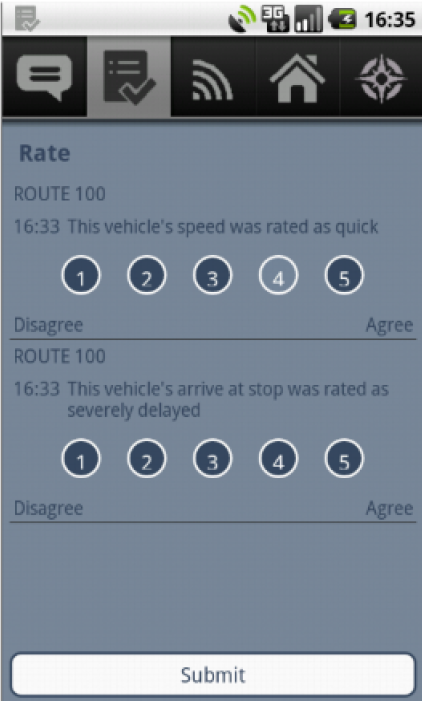
\includegraphics[scale=0.6]{rate_tab.png}
    \caption{Screenshot of the tab where we could find the rate comment feature.}
    \label{fig:rate_tab}
  \end{center}
\end{figure}

\pagebreak

All these questions and conclusions led to the development of a initial interface redesign, presented in the following section.

\section{Initial Proposals}\label{sec:initial}

After the initial process of perceiving what was done before, as well as understanding what were the advantages and disadvantages of the previous design decisions, and what went well and could go better, there was a group of decisions to be made concerning what the next steps would be. Those decisions consisted of:

\begin{itemize}
\item Technology - Despite being still on a premature phase, what technology would be used in order to develop the functional prototype? In this case, since that prototype is expected to be an \emph{Android} application, what would be the versions targeted for the prototype?

\item Main Navigation - How to design the main navigation for the application? Stick by the use of the tabs? Explore other solutions used in similar contexts? 

\item Information shown on User Profile - What is relevant to be shown to the user? Does the user wants to see nearby users? Is he willing to allow his location to be shared and to see where are the users generating useful information to them? Or does he want to focus on more personal information, such as possible rewards, points, statistics and so on?

\item Comment, Rate and News Feed features - Can these be aggregated in a way user understands or is familiar with, or it represents an excessive amount of information to be shown in one screen? 

\item Journey Planner features - Could other features with perceived utility to the user be added in order to allow a better comprehension of the concept behind the application, and consequently, a more efficient use (for instance, saving time and avoiding repetitive tasks)?
\end{itemize}

\subsection{Technology}
Some thought should be put on the first mentioned topic from the beginning, since the target version of the future application, apart from the possible conditioning of target users (who have outdated \emph{Android} versions on their devices), can influence the implemented interaction, since the newer versions of the operative system have several features related to animations, UI styling and interaction patterns.

The main decision was between sticking with a target version of \emph{Android} 2.x (however, using the API for version 2.3.3 instead of 2.2, because as of February 2014, \emph{Android} 2.2 (Froyo) users represented about only 1\% of all the \emph{Android} devices worldwide) or developing the prototype only for versions equal or superior to 4.0.3 (\emph{Ice Cream Sandwich)}. 

Despite the fact that the users of \emph{Android} versions inferior to 4.0.3 represent about 15\% of total \emph{Android} users, that number will surely reduce with the emergence of newer versions and devices. The 'time to market' of the application is expected to be wide, though, so it is expected that, when a fully implemented and improved version of the project is ready to be launched, those 15\% don't pose a limitation anymore. Apart from that fact, the advantage of developing the application for versions equal or superior to 4.0.3 is huge, because the API versions between \emph{Android} 3.0 and 4.0.3 introduced major improvements to the UI, text input and so on. 

Another important feature of this version is the Action Bar, used in the majority of \emph{Android} applications in order to serve as the main navigation menu of those applications, and that could be used as well in this project. The Action Bar menu came as a replacement for the Context Menu in older versions of \emph{Android}.

\clearpage

\begin{figure}[h!]
  \begin{center}
    \leavevmode
    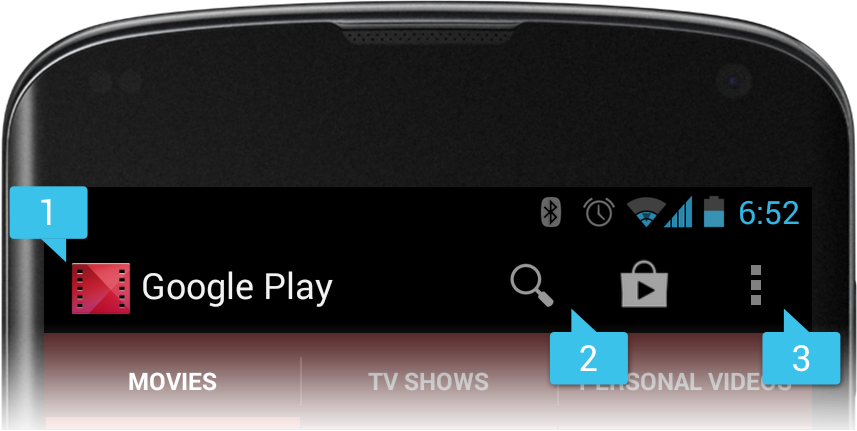
\includegraphics[scale=0.2]{actionbar.png}
    \caption{Example of an Action Bar from an \emph{Android} application, displaying the application icon (1), action items (2) and a menu option (3).}
    \label{fig:action}
  \end{center}
\end{figure}

It is also worth mentioning that one of the reasons of that change is the tendency to eliminate physical buttons from mobile devices (the first devices with \emph{Android} 4.0.3, such as \emph{Samsung Galaxy S III}, only had one physical button beneath the screen, resembling what happens with \emph{iOS} devices, and newer devices don't have a physical button beneath the screen at all).  

\subsection{Main Navigation}

About the main application navigation, the initial decision was to stick with a tab navigation, where a tab provided the access to one of the major features or modules of the application. However, there were several other questions that could be relevant:

\begin{itemize}
\item \emph{Screen position} - Top or bottom. Because we're talking about an \emph{Android} application, the best position would be top of the screen, since the recent versions of \emph{Android}, because of the already mentioned attempts to eliminate physical buttons on the devices, now has a bar on the bottom which has three buttons - \textbf{Back}, \textbf{Home} and \textbf{Recents} (this last one showing recently opened applications.

To put the tab navigation component could lead to user mistakes (touching the mentioned bar instead of the tab navigation). A tab navigation component in the bottom of the screen is, however, pretty common in \emph{iOS} mobile applications. 
There are a few cases where a navigation bar is placed in the bottom of the screen on \emph{Android}. For instance, when using the Action Bar for navigation, if there are a wide number of options that is desired to show to the user, it is possible to split the Action Bar, having the (usual) top one and another bar at the bottom. 


\end{itemize}

\begin{figure}[h!]
  \begin{center}
    \leavevmode
    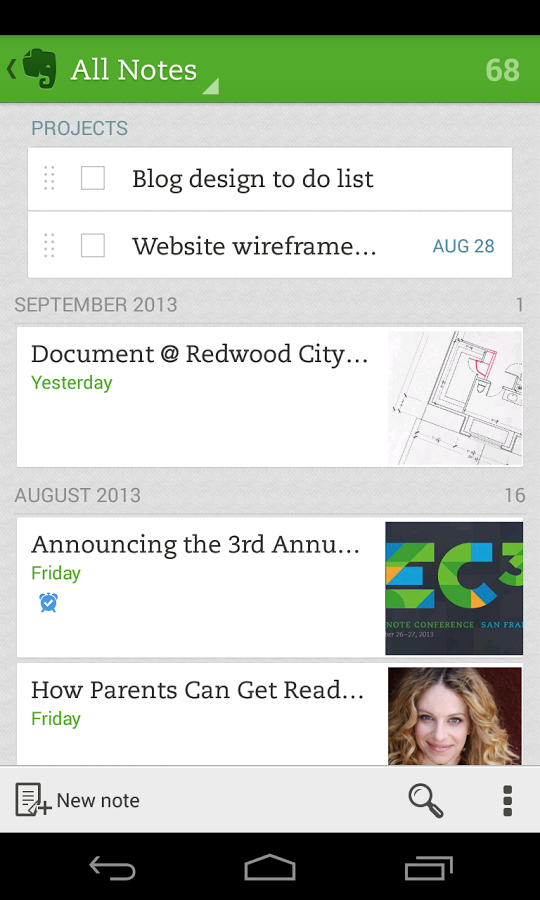
\includegraphics[scale=0.4]{evernote.png}
    \caption{Example of an application with splitted Action Bar - Evernote. Note also the bottom bar, present in recent devices.}
    \label{fig:evernote}
  \end{center}
\end{figure}

\begin{itemize}
\item \emph{Number of Tabs} - This number would depend on several factors. Visibility to the user is one of them. To have too many tabs, where some of them are initially hidden to the user (just accessible by using the swipe gesture, for instance) may cause those tabs and consequently the features they provide to be 'forgotten' and not as used as intended. 

In the work mentioned in the previous section, there were five tabs, all immediately visible to the user. This was perceived as an high number of tabs shown to the user. Reducing the number of visible (or total) tabs to three or four was explored in order to produce new design solutions.

\item \emph{Information displayed} - The previous prototype had icons representing each tab. There were no text labels displayed, and none of these icons is familiar to the user from similar contexts (applications or websites usage), apart from the icon from the fourth tab, intended to represent the tab containing the user profile. 

Metaphors that users associate with well-defined actions, pages, features or contexts, should not be used in order to represent different actions or contexts, because that will only confuse the user, improving the possibility of errors and confusion by the user. The biggest example of this is the 'save button'. An icon with a 3.5" floppy disk has been used for decades and has spread as representing the "save" action in a certain application. Today, despite the fact the younger generations don't recognise what a floppy disk is, they still associate the icon with saving.

In this case, the icon for the user profile tab as a house, usually associated with the existence of an Home screen or page. However, what was considered the 'Home tab' was in fact the user profile and not the start point of the application, and this issue could lead to errors or confusions from the user point of view.
\end{itemize}

Considering these points, two alternative designs were conceived for this component, all with four tabs - one with only three tabs visible at a given moment (the selected one should have a visible indicator in order to inform the user from that status), with no icons and just text labels \ref{fig:tabs1}; one with four fixed tabs (all visible), containing both icons and text labels \ref{fig:tabs2}. A slight variation of this one was also designed - with the addition of a coloured circle indicator to show the number of new items on the news feed list \ref{fig:tabs3}.

\begin{figure}[h!]
  \begin{center}
    \leavevmode
    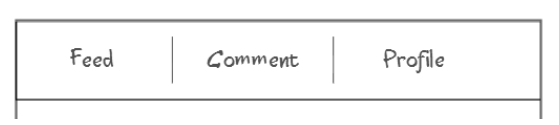
\includegraphics[scale=0.8]{tabs1.png}
    \caption{Initial draft of the tab component - three visible tabs, only text labels.}
    \label{fig:tabs1}
  \end{center}
\end{figure}

\begin{figure}[h!]
  \begin{center}
    \leavevmode
    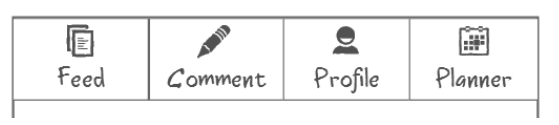
\includegraphics[scale=0.8]{tabs2.png}
    \caption{Initial draft of the tab component - four tabs, icons and text labels.}
    \label{fig:tabs2}
  \end{center}
\end{figure}

\begin{figure}[h!]
  \begin{center}
    \leavevmode
    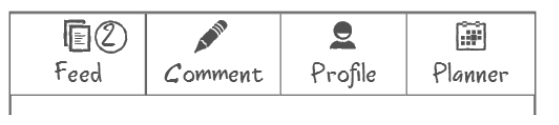
\includegraphics[scale=0.8]{tabs3.png}
    \caption{Initial draft of the tab component - four tabs, icons and text labels, and coloured indicator.}
    \label{fig:tabs3}
  \end{center}
\end{figure}

\subsection{User Profile}

The previous prototype gave the user the chance to check their points, stars and their username on their user profile, as well as change their nickname and a setting that allowed them to hide their nickname to other users. 

An additional button was also available, meant to fetch possible rewards that users could claim using points. Considering this, the displayed information was insufficient, too much free space remained vacant, and that space could be used in order to display other information the users of the application could find useful.

After an initial brainstorming session, there were several ideas about what sort of information could be displayed - user photo/avatar, a map of users in the same temporary network of the user (users who could contribute to the news feed that the user is receiving), information about the line and vehicle the user is in and a check-out button.

Two alternative designs were made, one with and one without the map with users in the same network. Since these initial designs were meant to act as a tool to wider the discussion on a focus group to be made (section \ref{sec:focusgroup}), the goal was to see if the users appreciated the idea of seeing other users (and their points) in the application, and if they were open to see their profile checked-out by other user (even if using the feature that allows to hide the real nickname).


\begin{figure}[h!]
  \begin{center}
    \leavevmode
    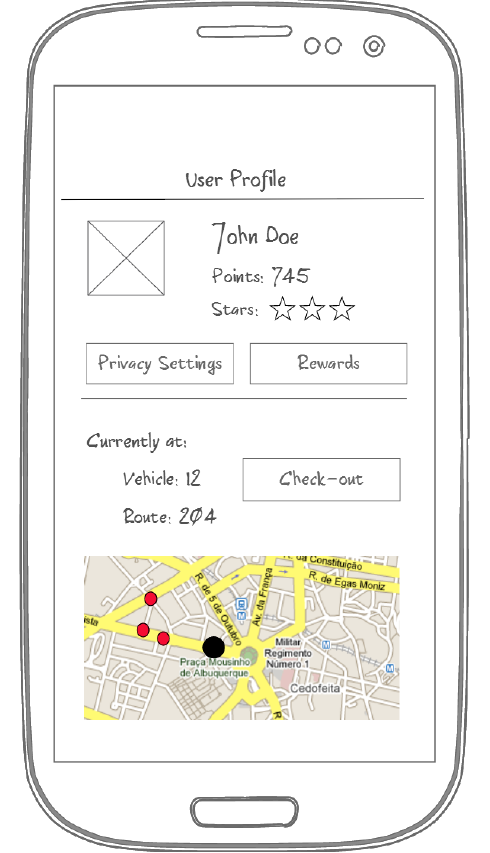
\includegraphics[scale=0.45]{profile1.png}
    \caption{Initial draft of the user profile screen - with network user map.}
    \label{fig:profile1}
  \end{center}
\end{figure}

For the first possibility (the one with the user map), it was also considered that a touch on a user on the map could display a dialog with a short profile of that user (username, points, stars and photo/avatar). That could, however, bring some usability difficulties due to the size of the elements that would represent a user on the map and would probably too small for this type of devices, where the touch gestures generally have low precision.

\begin{figure}[h!]
  \begin{center}
    \leavevmode
    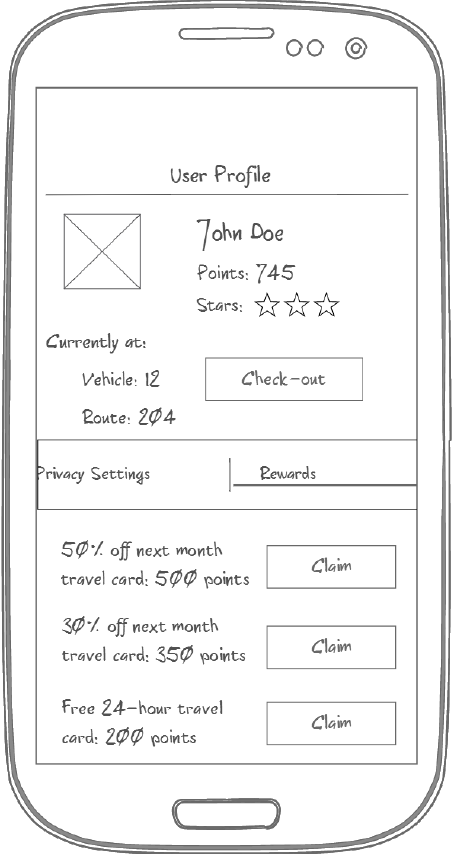
\includegraphics[scale=0.45]{profile2.png}
    \caption{Initial draft of the user profile screen - without network user map.}
    \label{fig:profile2}
  \end{center}
\end{figure}

\subsection{Comment, Rate and News Feed}

As said before, having the rate functionality separated from the news feed could have been the origin of the difficulty perceived by the users on grasping the feature. Explaining the feature in a more detailed way, after the submission of a comment by a user, that comment would be sent for two random people in the same network, who could verify the correctness of the information. 
The chosen users would then receive a notification informing them that there were comments left to rate. Only after successfully rated by two users, the comment would be published and available to other users in the network.

Two problems emerge from this system: first, there is the risk of an insufficient number of users in the network to perform the validation; second, because the comment would only be published after two successful ratings, there was also the risk that when those conditions were met the information would not be useful anymore.

The conceived solutions encompassed the aggregation of the rating feature with the news feed, with the 'must-rate' comments from other users appearing with a visual highlight (another background color, for example).
Both of those solutions involved as well showing the users' own comments in the news feed, aligned to the other side of the screen and also with a different background color to the message, resembling the behaviours usually seen in instant messaging or chat applications, that were since then applied to SMS applications on mobile devices.

The difference between the two solutions is that one of them includes the aggregation of the comment features in the news feed tab as well (joining the comment, rate and news feed features all-in-one), while the other maintains two distinct tabs, one for news feed and rating and another one for submitting a comment.

\begin{figure}[h!]
  \begin{center}
    \leavevmode
    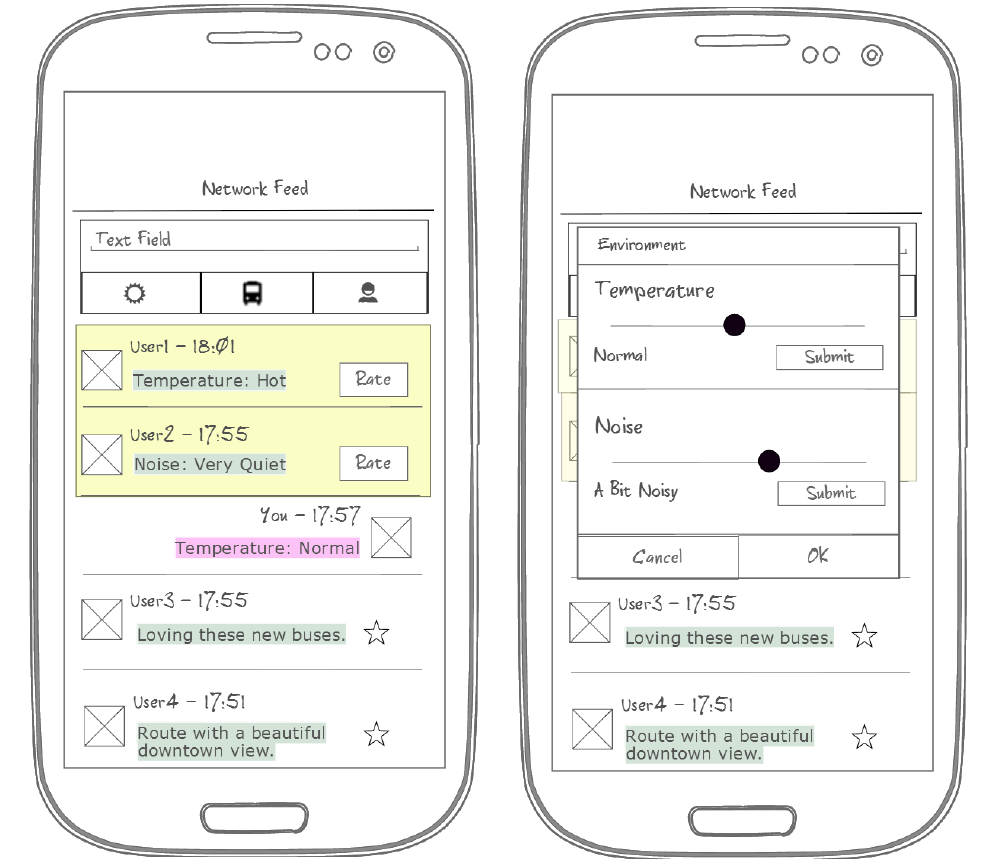
\includegraphics[scale=0.45]{comment2.png}
    \caption{Initial draft of the comment, rate and news feed features - all-in-one.}
    \label{fig:comment2}
  \end{center}
\end{figure}

\begin{figure}[h!]
  \begin{center}
    \leavevmode
    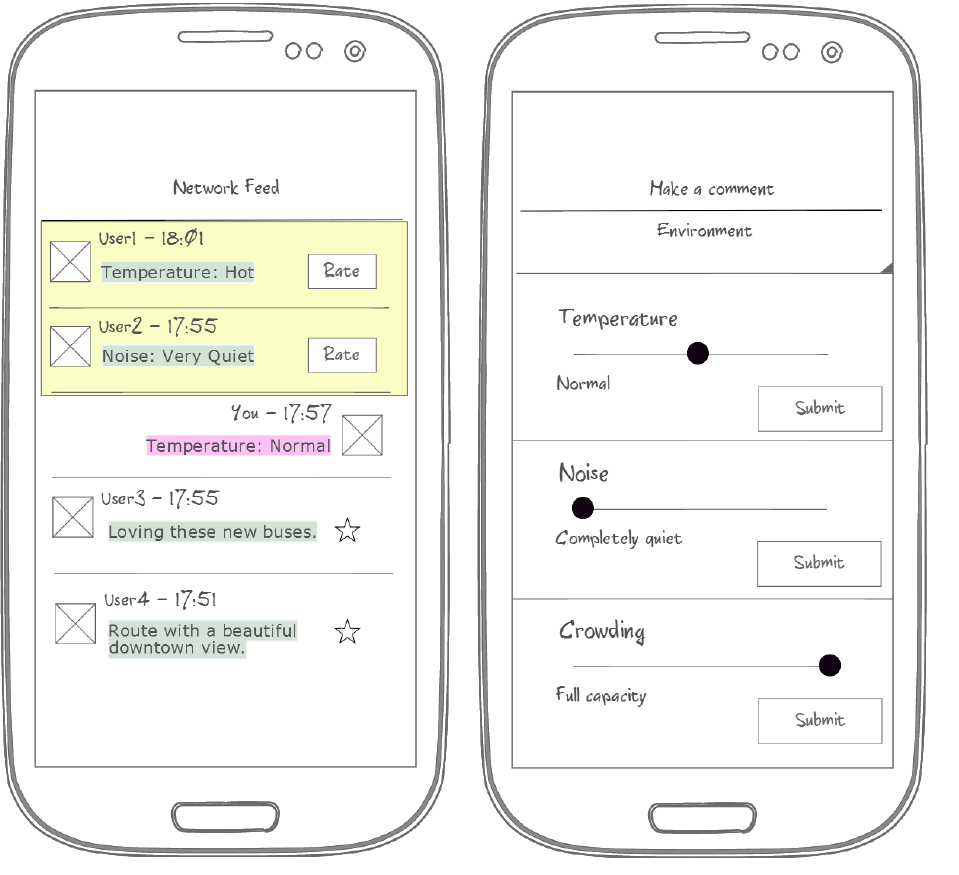
\includegraphics[scale=0.45]{comment1.png}
    \caption{Initial draft of the comment, rate and news feed features - news feed/rating aggregated, with comment in other tab.}
    \label{fig:comment1}
  \end{center}
\end{figure}

\subsection{Journey Planner}

The previous iteration of the project included a journey planner feature, that could be used by passengers to indicate trips they intend to make in the near future. Ten minutes before the chosen start time for the trip, the users would receive a notification reminding them of the planned trip and asking if they desire to receive information in real-time about the trip.

This feature has some importance in the application concept, because it may allow the system, in the future, to collect data related to the user trip profile, in order to predict, suggest and inform him about trips performed in a regular basis.

However, despite that possibility of planning a trip, after introducing that plan in the application, the user could not see the introduced plans. This was probably conceived this way to allow a user to plan just one trip for the next hour or so, but if a user wants to plan several trips for one day or week, there is no possibility of checking those trips, putting on the user all the effort to remind them.

Thus, a schedule feature was conceived, in order to give users that possibility, with the goal of catching their interest about the journey planner features.

The existing tab referring to the journey planner was maintained, adding one more screen to that tab (the schedule feature). That included the need for a secondary navigation that would allow the user to choose either the planner or the schedule tab. The considered solutions were a second set of tabs, or a spinner where the user could select the desired option.

\begin{figure}[h!]
  \begin{center}
    \leavevmode
    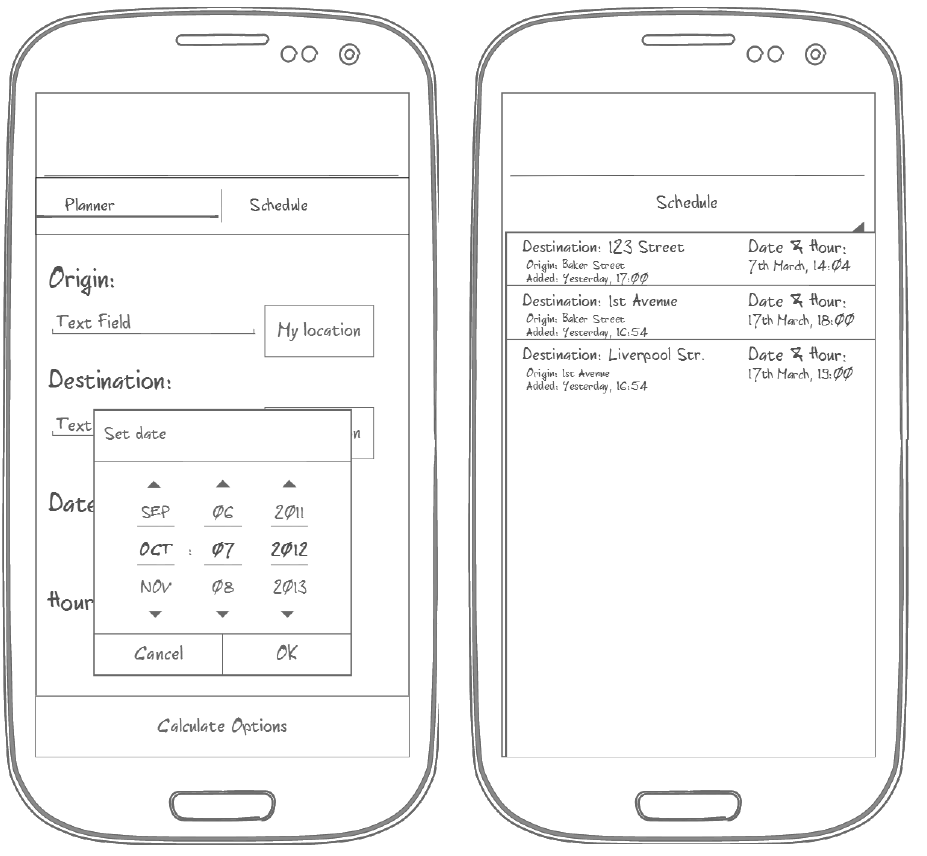
\includegraphics[scale=0.45]{planner1.png}
    \caption{Initial draft of the journey planner features - with tabs on the left, with spinners on the right.}
    \label{fig:planner1}
  \end{center}
\end{figure}

\section{Focus Group}\label{focusgroup}

During this phase, in order to define and specify usability requirements, a focus group session was held at \emph{IBM-CAS} room at FEUP.

Focus groups consist in an informal technique used to understand user needs and feelings. This technique can be used at any stage of the development phase, before the design phase or even after the implementation, with the goal of discussing issues and concerns about  the features of an user interface. 

These sessions usually bring together between six and nine users, typically lasting about two hours. A moderator should be assigned to the session, in order to maintain the group's focus \cite{kn: Nielsen07}. 

In this case, the main goal for the session held was to understand what users needed, presenting them the alternatives mentioned on the previous section to discussion. Note that these kind of sessions are not intended to evaluate interface usability (because usually participants do not have the chance to use the product on their own, but instead a demo is presented to the whole group). In this particular case, it was intended to check if the application could solve some of the users' problems regarding public transport information, what could be done to improve that matter and changes regarding the interaction that could lead to that improvement.

Six participants with different backgrounds, age groups and different patterns of public transport use were part of the session. In Table \ref{table:table1}, is it possible to see those characteristics in more detail.

\begin{table}{t}

\begin{center}
\begin{tabular}{ c c c c p{5cm} }

  \hline 
  \textbf{\#} & \textbf{Gender} & \textbf{Age Group} & \textbf{Public transport usage profile} & \textbf{Background} \\
  \hline 
  1 & Male & 18-30 & Frequent subway user & Public transport related Msc. thesis
   student \\
  \hline
  2 & Female & 18-30 & Occasional bus and subway user & HCI related Msc. thesis student \\
  \hline
  3 & Male & 40-60 & Occasional bus and subway user & 20+ years experience with public transport
  network studies (customer satisfaction
   and scheduling) \\ 
  \hline
  4 & Male & 18-30 & Frequent bus and subway user & Msc. Student in Services Engineering
   and Management\\
  \hline
  5 & Male & 30-40 & Occasional bus and subway user & PhD. Researcher in public transport
   networks field\\
  \hline
  6 & Female & 40-60 & Occasional bus and subway user & PhD. in Operations Research\\
  \hline
\end{tabular}
\caption{Focus group participants characteristics.}
\label{tab:table1}
\end{center}
\end{table}


